\documentclass{article}
\usepackage[utf8]{inputenc}
\usepackage{graphicx}
\usepackage{amsmath}
\usepackage{float}
\usepackage{indentfirst}
\usepackage{biblatex}
\addbibresource{database.bib}
\numberwithin{equation}{section}


\graphicspath{ {images/} }

\title{Semester Project}
\author{Brett Stephens }
\date{December 2017}
\begin{document}
\maketitle
The following documentation includes the derivation process required to map steering angles and determine tire parameters for the Zürich Autonomous Race Car (ZARC).
\section{Steering Angle Identification}
In order to map the commanded pulse width modulated (pwm) signal from a controller to a steering angle, a deeper understanding of the vehicle kinematics was needed.   
\begin{figure}[H]
\centering
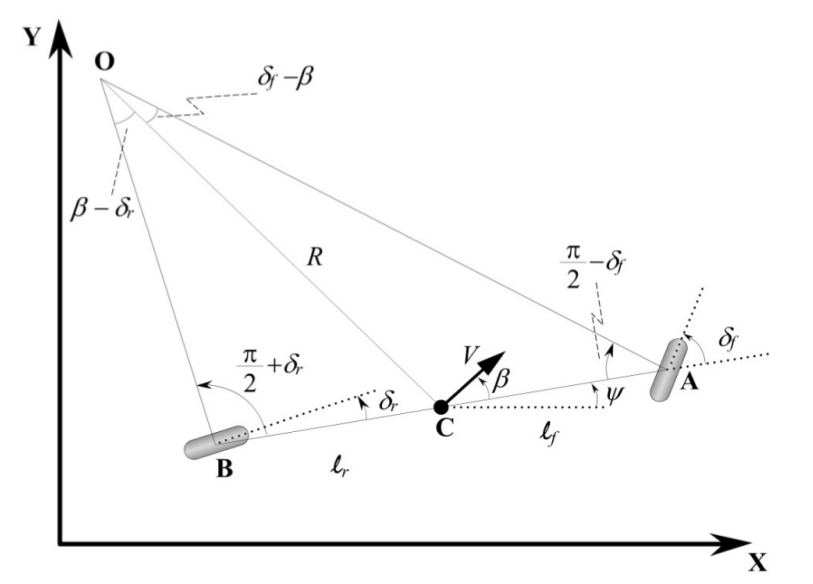
\includegraphics[width=8cm]{BicycleModel.png}
\caption{Kinemtic Bicycle Model}
\label{fig:BicycleModel}
\end{figure}
\begin{flushleft}
Using a simple kinematic bicycle model (with $\delta_r = 0$), the following relations can be derived. 
Looking at triangle OCA:
\end{flushleft}
\begin{equation} \label{eq1.1}
    \frac{sin(\delta_f - \beta)}{l_f} = \frac{sin(\pi/2 -\delta_f)}{R}
\end{equation}
And triangle OCB:
\begin{equation} \label{eq1.2}
    \frac{sin(\beta)}{l_r} = \frac{sin(\pi/2)}{R}
\end{equation}
Using trigonometric identities, \eqref{eq1.1} becomes:
\begin{equation} \label{eq1.3}
    \frac{sin(\delta_f)cos(\beta)-sin(\beta)cos(\delta_f)}{l_f} = \frac{cos(\delta_f)}{R}
\end{equation}
And \eqref{eq1.2} simplifies to:
\begin{equation}\label{eq1.4}
    \frac{sin(\beta)}{l_r} = \frac{1}{R}
\end{equation}
Combining \eqref{eq1.3} and \eqref{eq1.4}:
\begin{equation} \label{eq1.5}
    tan(\delta_f)cos(\beta) = \frac{l_r+l_f}{R}
\end{equation}
With a low constant velocity, vehicle lateral velocity $V_y$ can be approximated to 0. As such $\cos(\beta)\approx{1}$. 
Additionally, with a constant steering angle $\delta_f$, the change in orientation of the vehicle ($\dot{\Psi}$) is equal to the angular velocity of the vehicle:
\begin{equation}\label{eq1.6}
    \dot{\Psi} = \omega = \frac{V}{R}
\end{equation}
Lastly, by combining \eqref{eq1.5} and \eqref{eq1.6}, a relation for the steering angle is found:
\begin{equation}\label{eq1.7}
    \delta_f = \arctan\bigg(\frac{\dot{\Psi}(l_r+l_f)}{V}\bigg)
\end{equation}
Keeping a low constant velocity, the parameters of \eqref{eq1.7} were measured with a Vicon motion capture system for a variety of constant steering angles $\delta_f$. For each $\delta_f$, the gathered parameter data was averaged: 
\begin{figure}[H]
\centering
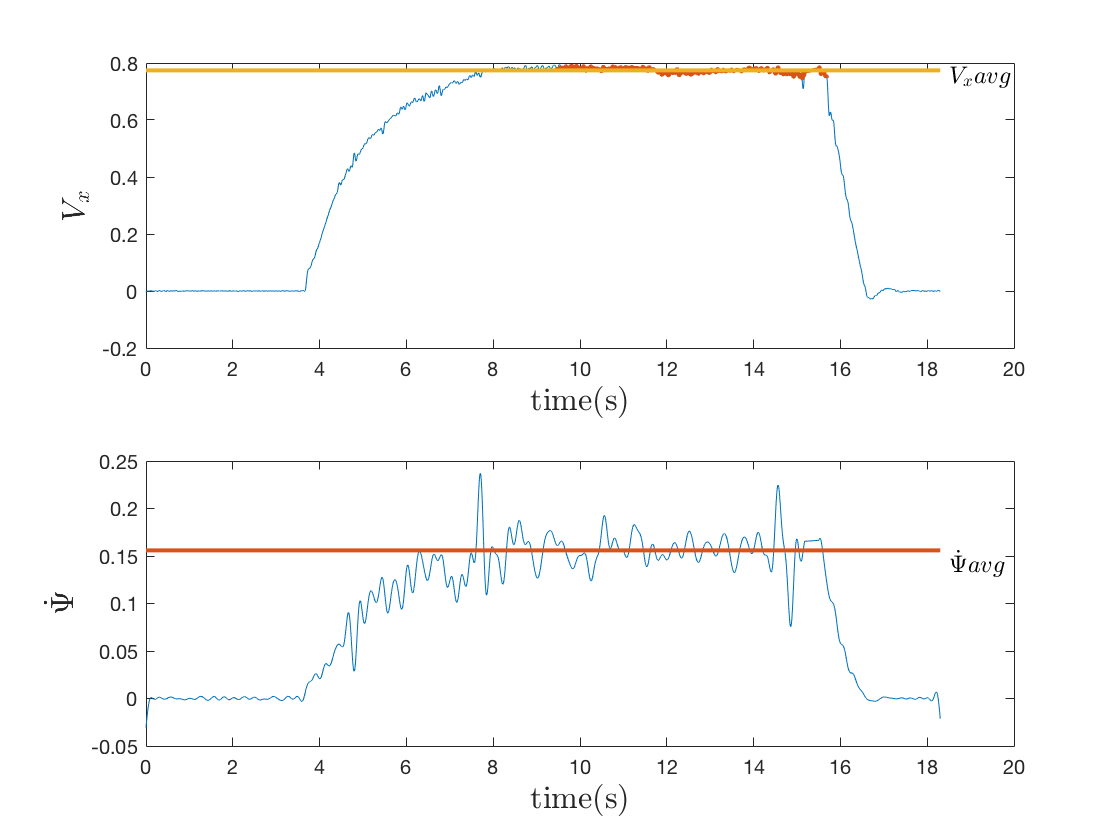
\includegraphics[width=8cm]{VelAVG.png}
\caption{Average longitudinal velocity and yaw rate}
\label{fig:VelAVG}
\end{figure}
Which then led to the generation of the following map:
\begin{figure}[H]
\centering
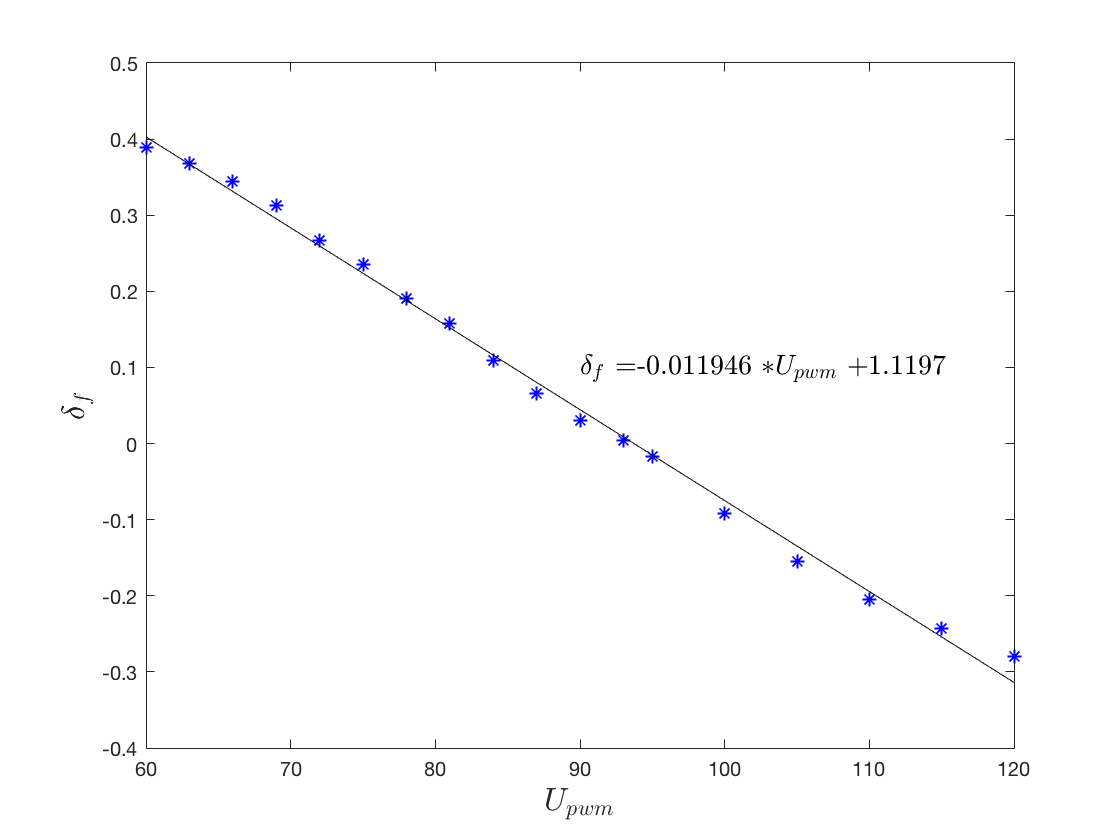
\includegraphics[width=8cm]{SteeringMapping.png}
\caption{Steering Angle Map}
\label{fig:SteeringMap}
\end{figure}

\begin{flushleft}
The following linear relation between $\delta_f$ and $U_{pwm}$ was found to be $\delta_f = -0.0119U_{pwm} + 1.119$.
\end{flushleft}

\section{Tire Parameter Identification}

To gain further insight into the vehicle's dynamics, the tire behavior must be considered. Understanding the conditions under which the front and rear tires become saturated is essential to predict when a slip or drift condition will occur. A test known as ramp steer can be performed in order to generate a lateral force vs slip angle curve. For this test, the vehicle turns with a linearly increasing steering angle while the forward velocity remains constant. If the steering angle is increased slowly, steady state cornering can be assumed. 

With this test, two important tire characteristics can be found: the linear relationship between lateral tire force and slip angle at small slip angles, and tire saturation due to friction limitations. Again, using a bicycle model, the following method was utilized:
\begin{figure}[H]
\centering
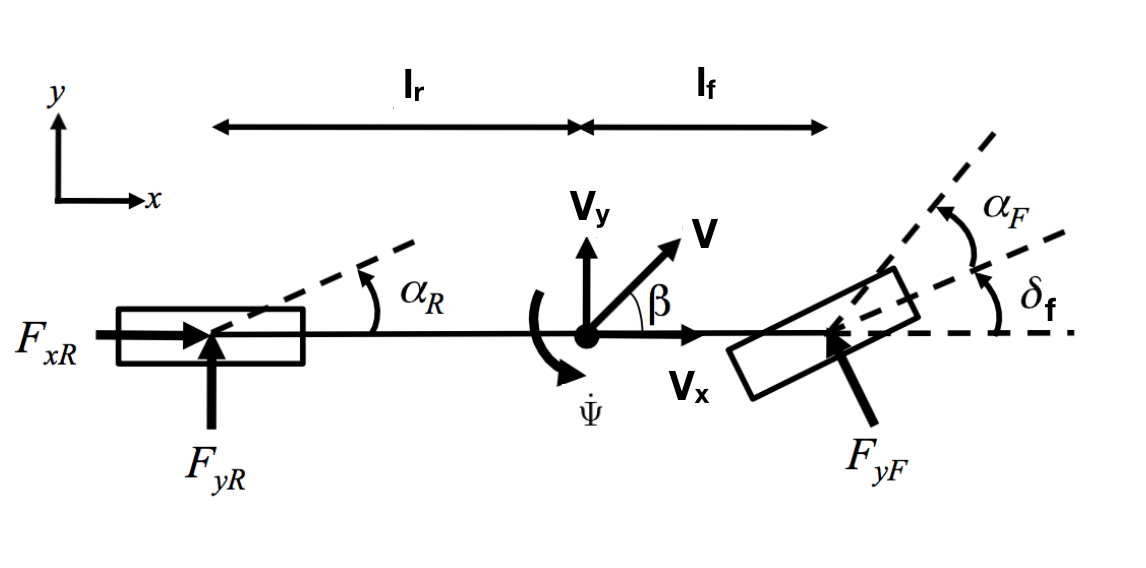
\includegraphics[width=8cm]{BikeModelK.png}
\caption{Dynamic Bicycle Model}
\label{fig:BikeModelK}
\end{figure}
By performing a sum of forces in the y-direction and a sum of moments about the z-axis, the following relations are derived:
\begin{equation}\label{eq2.1}
    ma_y = F_{yF}\cos{\delta_f} + F_{yR}
\end{equation}
\begin{equation}\label{eq2.2}
    I_z\ddot{\Psi} = l_fF_{yF}\cos{\delta_f} - l_rF_{yR}
\end{equation}
An expression for $a_y$ in \eqref{eq2.1} can be found:
\begin{equation}\label{eq2.3}
    a_y = \dot{V_y} + \dot{\Psi} V_x
\end{equation}
Substituting \eqref{eq2.3} into \eqref{eq2.1} and assuming $\delta_f$ to be small ($\cos{\delta_f}\approx{1}$):
\begin{equation}\label{eq2.4}
    \dot{V_y} = \frac{F_{yF}+F_{yR}}{m} - \dot{\Psi} V_x
\end{equation}
\begin{equation}\label{eq2.5}
    \ddot{\Psi} = \frac{l_f F_{yF} - l_r F_{yR}}{I_z}
\end{equation}
The above relations can be expressed in terms of $\beta$, the side slip angle, which often used to characterize drift. Using the small angle approximation, $\beta = \arctan\frac{V_y}{V_x}\approx{\frac{V_y}{V_x}}$
and $\dot{\beta}\approx{\frac{\dot{V_y}}{V_x}}$, the expression in \eqref{eq2.4} can be updated to:
\begin{equation}\label{eq2.6}
    \dot{\beta} = \frac{F_{yF} + F_{yR}}{mU_x} - \dot{\Psi}
\end{equation}
As stated previously, the ramp steer test maintains steady state cornering and as such, $\dot{\beta} = \ddot{\Psi} = 0$. Combining this with \eqref{eq2.5} and \eqref{eq2.6}, and solving for the lateral forces, we arrive at the following:
\begin{equation}\label{eq2.7}
    F_{yF} = \frac{l_r}{L}ma_y^{SS}
\end{equation}
\begin{equation}\label{eq2.8}
    F_{yR} = \frac{l_f}{L}ma_y^{SS}
\end{equation}
Where $a_y^{SS}$ is the steady state lateral acceleration defined as $a_y^{SS} = \dot{\Psi} V_x$ and $L$ is the vehicle wheel base.
Lastly, an expression for the front and rear slip angles must be found. Looking at figure \ref{fig:BikeModelK}, the expression is determined to be
\begin{equation}\label{eq2.9}
    \alpha_F = \arctan\frac{V_y + l_f \dot{\Psi}}{V_x} - \delta_f \approx{\arctan\bigg(\beta + \frac{l_f}{V_x}\dot{\Psi}\bigg)-\delta_f}
\end{equation}
\begin{equation}\label{eq2.10}
    \alpha_R = \arctan\frac{V_y - l_r \dot{\Psi}}{V_x}\approx{\arctan\bigg(\beta - \frac{l_r}{V_x}\dot{\Psi}\bigg)}
\end{equation}
Using relations \eqref{eq2.7}, \eqref{eq2.8} along with \eqref{eq2.9}, \eqref{eq2.10}, it is possible to empirically derive a lateral force vs slip angle plot for a linearly increasing steering angle $\delta_f$.

In order to implement a vehicle controller, it is useful to generate a model to fit the empirical data. In order to do so, a brush tire model is used. The following figures and derivations are sourced from \cite{Hindiyeh}. 
The brush tire model divides the tire into several parts,including a rectangular patch of the tire which contacts the road. The patch is defined by "brushes", which populate the portion of the tire in contact the road and span a length of $2l$. When a cornering maneuver occurs, the lateral force required for a successful turn is a result of the tire slip angle $\alpha$ as seen in \ref{fig:SlipAngle}. 
\begin{figure}[H]
\centering
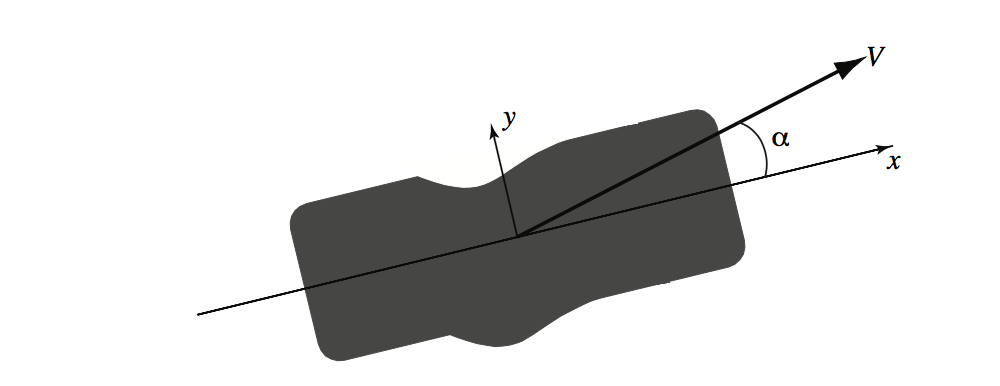
\includegraphics[width=8cm]{SlipAngle.png}
\caption{Tire Slip Angle}
\label{fig:SlipAngle}
\end{figure}
The lateral force profile therefore takes the following shape:
\begin{figure}[H]
\centering
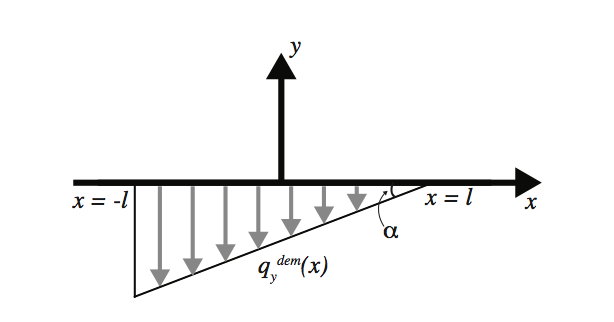
\includegraphics[width=8cm]{LatForceProfile.png}
\caption{Tire Slip Angle}
\label{fig:LatForceProfile}
\end{figure}
\ref{fig:LatForceProfile} can be described mathematically by
\begin{equation}\label{eq2.11}
    q_y^{dem}(x) = -c_{py}(a-x)\tanh{\alpha}
\end{equation}
The lateral force available from the tire is a function of the normal force acting on the tire in the z direction and the coefficient of friction between the contact patch and the ground. The normal force can be modeled as a quadratic function of position x from the center of the contact patch:
\begin{equation}\label{eq2.12}
    q_z(x) = \frac{3F_z}{4l}\bigg(\frac{l^2-x^2}{l^2}\bigg),
\end{equation}
$F_z$ is the total normal force on the tire when $q_z(x)$ is integrated across the contact patch length. A graphical representation can be seen below.
\begin{figure}[H]
\centering
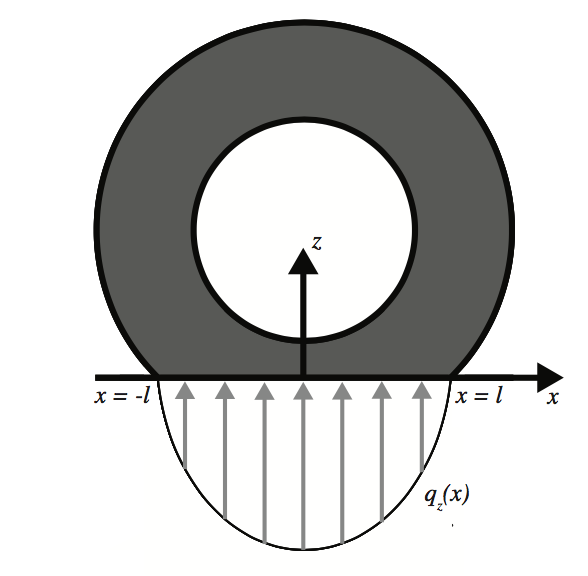
\includegraphics[width=8cm]{NormalTireProfile.png}
\caption{Normal Force Tire Profile}
\label{fig:NormalTireProfile}
\end{figure}
The total force that is available from friction is $\mu q_z(x)$ and therefore the following relation can be defined:
\begin{equation}\label{eq2.13}
    |q_y(x)|\leq\mu q_z(x)
\end{equation}
A graphical representation of this is found below, where the tire slip angle is increasing to the right.
\begin{figure}[H]
\centering
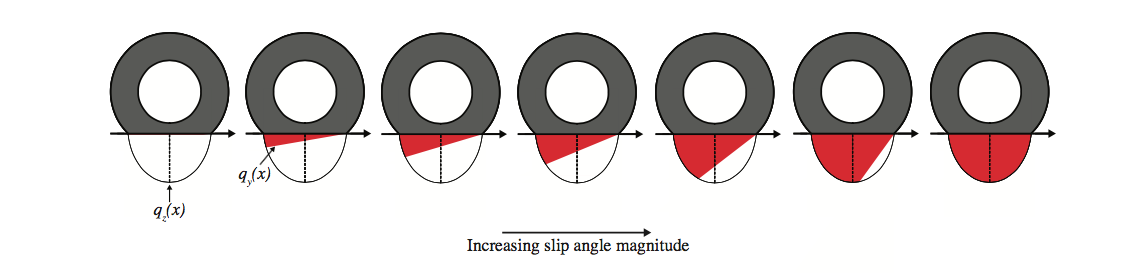
\includegraphics[width=12cm]{IncreasingSlip.png}
\caption{Tire Slip Angle Progression}
\label{fig:IncreasingSlip}
\end{figure}
Looking at \ref{fig:IncreasingSlip}, it can be seen that the "rear" of the contact patch begins to intersect the normal force parabola defined by $q_z(x)$. Ahead of this intersection, $q_y$ = $q_y^{dem}(x)$, meaning the the tire is able to accommodate the requested lateral force. Behind this intersection, however, $q_y$ exceeds the force "availability" of the tire and becomes friction-limited, in that $q_y = \mu q_z$. This saturation point can be clearly seen in a typical lateral force vs slip angle curve as the initial linear behavior of the curve begins to level off at a constant lateral force. This "flat" portion is characterized by the far right animation of \ref{fig:IncreasingSlip}. 

Lastly, $q_y(x)$ can be integrated in order to produce a relation for $F_y$ as a  function of slip angle $\alpha$:
\begin{equation}\label{eq2.14}
F_y =
\begin{cases} 
      -C_\alpha\tan{\alpha} + 
       \frac{C_\alpha^2}{3\mu F_z}|\tan{\alpha}|\tan{\alpha} - \frac{C_\alpha^3}{27\mu^2 F_z^2}\tan^3{\alpha}, & \text{if $|\alpha|\leq\alpha_{sl}$},\\
      -\mu F_z sgn\alpha, & \text{otherwise}
   \end{cases}
\end{equation}
Where $C_\alpha = 2c_{py}l^2$ is the cornering stiffness of the tire and  $\alpha_{sl}$ is the smallest slip angle for which the entire tire is saturated as seen in the rightmost image in figure \ref{fig:IncreasingSlip}. $\alpha_{sl}$ can be found to be:
\begin{equation}\label{eq2.15}
    \alpha_{sl} = \arctan{\frac{3\mu F_z}{C_\alpha}}
\end{equation}
From \eqref{eq2.14}, a line fitting the emperical data can be obtained.

\renewcommand{\arraystretch}{1.5}
\begin{table}[H]
\centering
 \begin{tabular}{ |c|c|  }
 \hline
 \multicolumn{2}{|c|}{Vehicle Parameters} \\
 \hline
 Parameter & Value \\ [0.5ex] 
 \hline
 $F_{zF}$ & 12.6941 N \\ 
 $F_{rF}$ & 14.7454 N \\
 $l_f$ & 0.1741 m\\
 $l_r$ & 0.1499 m\\
 $m$ & 2.792 kg \\ [1ex] 
 \hline
 \end{tabular}
\end{table}

\begin{table}[H]
\centering
 \begin{tabular}{ |c|c|  }
 \hline
 \multicolumn{2}{|c|}{Tire Model} \\
 \hline
 States &  $\beta,\dot{\Psi}$\\ 
 Input & $\delta_f$ \\ [1ex] 
 \hline
 \end{tabular}
\end{table}



\printbibliography %Prints bibliography

\end{document}